\documentclass[UTF8]{ctexart}
\usepackage{geometry, CJKutf8}
\geometry{margin=1.5cm, vmargin={0pt,1cm}}
\setlength{\topmargin}{-1cm}
\setlength{\paperheight}{29.7cm}
\setlength{\textheight}{25.3cm}
\usepackage[dvipsnames]{xcolor}
% useful packages.
\usepackage{amsfonts}
\usepackage{amsmath}
\usepackage{amssymb}
\usepackage{amsthm}
\usepackage{enumerate}
\usepackage{graphicx}
\usepackage{multicol}
\usepackage{fancyhdr}
\usepackage{layout}
\usepackage{listings}
\usepackage{float, caption}
\usepackage{bm}
\usepackage{booktabs}  
\usepackage{array}   
\lstset{
    basicstyle=\ttfamily, basewidth=0.5em
}

\newcommand{\dif}{\mathrm{d}}
\newcommand{\avg}[1]{\left\langle #1 \right\rangle}
\newcommand{\difFrac}[2]{\frac{\dif #1}{\dif #2}}
\newcommand{\pdfFrac}[2]{\frac{\partial #1}{\partial #2}}
\newcommand{\OFL}{\mathrm{OFL}}
\newcommand{\UFL}{\mathrm{UFL}}
\newcommand{\fl}{\mathrm{fl}}
\newcommand{\op}{\odot}
\newcommand{\Eabs}{E_{\mathrm{abs}}}
\newcommand{\Erel}{E_{\mathrm{rel}}}

\begin{document}

\pagestyle{fancy}
\fancyhead{}
\lhead{张子乐, 3230104237}
\chead{非参数密度函数估计的收敛速度}
\rhead{March.4th, 2026}

\section{直方图估计}

\subsection{定义}

一般情况下多维直方图估计的定义为
\begin{equation}
\hat{p}_H(y) = 
\begin{cases} 
\sum_{k=1}^m \frac{1}{v_k} \frac{\sum_{i=1}^n I_{T_k}(y_i)}{n} I_{T_k}(y), & \text{for } y \in D; \\ 
0, & \text{otherwise}. 
\end{cases}
\end{equation}

其中$D$是概率密度函数的有限支撑集，
$m$是区间的数量，
$T_k$表示第 $k$ 个区间，
$v_k$表示第 $k$ 个区间的体积（在单变量中代表长度 $h_k$，在二维中代表面积），
$n$表示总样本量，
$y_i$表示第 $i$ 个观测样本。

令 $n_k = \sum_{i=1}^n I_{T_k}(y_i)$ 表示落入第 $k$ 个区间中的样本数量，
则上述定义简化为：
\begin{equation}
\hat{p}_H(y) = \sum_{k=1}^m \frac{n_k}{n v_k} I_{T_k}(y)
\end{equation}

一维情况下用$t_{n,k+1} - t_{n,k}$表示第 $k$ 个区间的长度：
\begin{equation}
\hat{p}_H(y) = \sum_{k=1}^m \frac{n_k}{n(t_{n,k+1} - t_{n,k})} I_{T_k}(y)
\end{equation}

若固定区间长度为 $h$，则上述定义进一步简化为：
\begin{equation}
\hat{p}_H(y) = \frac{n_k}{nh}, \quad \text{for } y \in T_k
\end{equation}

\subsection{直方图估计的均方误差}

第k个区间中的点y的直方图估计的均方误差由下式给出：
\begin{equation}
\text{MSE}(\hat{p}_H(y)) = \frac{p_k(1-p_k)}{nv_k^2} + \left( \frac{p_k}{v_k} - p(y) \right)^2
\end{equation}

其由两部分组成，分别为样本落在区间内(服从二项分布)的方差和密度估计与真实密度偏差的平方。

直方图估计的数学期望是$E(\hat{p}_H(y)) = \frac{p_k}{v_k}$，
因此偏差项为$\frac{p_k}{v_k} - p(y)$。
若真实密度函数满足 Lipschitz 连续：$|p(y_1) - p(y_2)| \le \gamma_k |y_1 - y_2|$，
则偏差项的上界为$ \gamma_k v_k$。

直方图估计的方差为
\begin{equation}
    V(\hat{p}_H(y)) = V(n_k) / (n v_k)^2 = p_k(1-p_k) / (n v_k^2)
\end{equation}

其中$n_k$服从参数为$n$和$p_k$的二项分布.
利用积分中值定理，$V(\hat{p}_H(y)) \le \frac{p(\xi_k)}{nv_k}$，
其中$\xi_k$第k个区间中的某一点。
由此也能看出方差与偏差的权衡，当区间宽度增加时，偏差会增加但方差会减少。

由此，均方误差放缩为下式：
\begin{equation}
\text{MSE}(\hat{p}_H(y)) \le \frac{p(\xi_k)}{nv_k} + \gamma_k^2 v_k^2
\end{equation}

为最小化均方误差，对区间宽度求导并令其为零，解得：
\begin{equation}
h^*(k) = \left( \frac{p(\xi_k)}{2\gamma_k^2 n} \right)^{1/3}
\end{equation}

这表明，区间宽度应以 $\mathcal{O}(n^{-1/3})$ 的速度衰减，
此时均方误差量级为：
\begin{equation}
\text{MSE}^*(\hat{p}_H(y)) = \mathcal{O}(n^{-2/3})
\end{equation}

即直方图估计该点逼近真实密度函数的收敛速度为 $\mathcal{O}(n^{-1/3})$。

\subsection{渐进均方积分误差AMISE}

上面计算的是在某一点的均方误差，
下面计算渐近均方积分误差（AMISE）评估全局误差。
论文中考虑的是多维的情况。

假设所有矩形箱的各个维度边长恒定为 $h_1, \dots, h_d$，
且体积为 $v = \prod_{j=1}^d h_j$。

分别对方差和偏差进行积分，并舍去高阶无关项，
得到渐进方差和渐进平方偏差：
\begin{align}
\text{AIV}(\hat{p}_H) &= \frac{1}{nv} = \frac{1}{n(h_1 \cdots h_d)} \\
\text{AISB}(\hat{p}_H) &= \frac{1}{12} \sum_{j=1}^d h_j^2 R(\nabla_j p)
\end{align}

其中，$R(\nabla_j p)$ 表示
真实密度函数在第 $j$ 个维度上梯度的“roughness”：$R(g) = \int_{\mathbb{R}^d} g(t)^2 \, \mathrm{d}t$.

相加得到渐进均方积分误差：
\begin{equation}
\text{AMISE}(\hat{p}_H) = \frac{1}{n(h_1 \cdots h_d)} + \frac{1}{12} \sum_{j=1}^d h_j^2 R(\nabla_j p)
\end{equation}

对 AMISE 公式关于 $h_j$ 求导并令其为零：
\begin{equation}
    h_{j*} = R(\nabla_j p)^{-1/2} \left( 6 \prod_{i=1}^d R(\nabla_i p)^{1/2} \right)^{\frac{1}{2+d}} n^{-\frac{1}{2+d}}
\end{equation}

此时渐进均方积分误差的衰减速率为：
\begin{equation}
\text{AMISE}^*(\hat{p}_H) = \mathcal{O}\left(n^{-\frac{2}{2+d}}\right)
\end{equation}

但是，
$h_{j*}$ 的表达式中包含了真实密度函数的$R(\nabla_j p)$，
它应该是未知的。

不妨假设真实分布是一个"good general distribution"，
即协方差阵为对角矩阵$\Sigma = \text{diag}(\sigma_1^2, \dots, \sigma_d^2)$的d维正态分布，
此时$R(\nabla_j p) = \frac{1}{2^{d+1} \pi^{d/2} \sigma_j^2 \left|\Sigma^{1/2}\right|}$。


一维情况下,$R(p') = 1/(4\sqrt{\pi}\sigma^3)$，
代入即得$h^* = 3.49 \sigma n^{-1/3}$。
在实际计算中，可以使用样本标准差 $s$ 来代替总体标准差 $\sigma$。

相比设定直方图区间的宽度，
直接设定直方图区间的数量往往更多的被使用。
假设直方图的区间数服从一个对称的二项分布模型，
有：
\begin{equation}
    n = \sum_{k=0}^{m-1} \binom{m-1}{k}  = 2^{m-1}.
\end{equation}

可以取区间的数量$m = 1 + \log_2 n$。

\section{核密度估计}

\subsection{Rosenblatt直方图估计与核密度估计}

一维情况下，上面的直方图估计区间位置是固定的，
Rosenblatt直方图估计则以目标点 $y$ 为中心，
向两侧各延伸 $h/2$ 的距离构建一个动态区间，
统计落入该区间 $(y - h/2, y + h/2]$ 内的样本点数量：
\begin{equation}
\hat{p}_R(y) = \frac{\#\{y_i : y_i \in (y - h/2, y + h/2]\}}{nh}
\end{equation}

其可以等价地表示为经验分布函数的形式：
\begin{equation}
\hat{p}_R(y) = \frac{P_n(y + h/2) - P_n(y - h/2)}{h}
\end{equation}

若改写为针对每个样本点 $y_i$ 的求和形式：
\begin{equation}
\hat{p}_R(y) = \frac{1}{nh} \sum_{i=1}^n K\left(\frac{y - y_i}{h}\right)
\end{equation}

其中，这里函数 $K_1(x)$ 的定义为：当 $|x| < 1/2$ 时，$K_1(x) = 1$；否则 $K_1(x) = 0$。
$K(x)$也可以取其它的核函数，这便是核密度估计的一般形式。

例如：
\begin{align*}
K_2(x) &= (1-|x|)I_{[-1,1]}(x) \quad \text{(三角形核)} \\
K_3(x) &= \frac{3}{4}(1-x^2)I_{[-1,1]}(x) \quad \text{(二次曲线核)} \\
K_4(x) &= \frac{15}{16}(1-x^2)^2I_{[-1,1]}(x) \quad \text{(双二次核)} \\
K_5(x) &= \frac{70}{81}(1-|x|^3)^3I_{[-1,1]}(x) \quad \text{(双三次核)} \\
K_6(x) &= \frac{1}{\sqrt{2\pi}}e^{-\frac{x^2}{2}} \quad \text{(高斯核)}
\end{align*}

一般地，核函数应该满足如下要求:
\begin{enumerate}
    \item $K(x) \ge 0$;
    \item $\int_{-\infty}^{\infty} K(x)dx = 1$;
    \item $K(x)$ 是偶函数;
    \item $\int_{-\infty}^{\infty} x^2 K(x)dx < +\infty$ 。
\end{enumerate}

可以利用这些性质来推导核密度估计的偏差和方差。

\subsection{核密度估计的理论性质}

在Emanuel Parzen 1962年发表的论文
On Estimation of a Probability Density Function and Mode中，作者
详细推导了核密度估计的理论性质。

\subsubsection{渐进无偏性}

当$h(n)$ 满足 $h(n) > 0$ 且 $\lim_{n \rightarrow \infty} h(n) = 0$，
且核函数$K(y)$
绝对有界且可积 $\sup |K(y)| < \infty$、$\int |K(y)|dy < \infty$，以及
$\lim_{y \rightarrow \infty} |yK(y)| = 0$时，
有：
\begin{equation}
E[f_n(x)] = \int_{-\infty}^{\infty} \frac{1}{h(n)} K\left(\frac{x-y}{h(n)}\right) f(y) dy
\end{equation}

对于真实密度函数 $f(x)$ 的任意连续点 $x$，均有：
\begin{equation}
\lim_{n \rightarrow \infty} E[f_n(x)] = f(x)
\end{equation}

这说明了以上条件下核密度估计是真实密度函数的渐近无偏估计。

\subsubsection{均方一致性}

估计量的均方误差可分解为方差与偏差的平方和：
\begin{equation}
E|f_n(x) - f(x)|^2 = \text{Var}[f_n(x)] + b^2[f_n(x)]
\end{equation}

论文给出了方差的极限：
\begin{equation}
\lim_{n \rightarrow \infty} n h(n) \text{Var}[f_n(x)] = f(x) \int_{-\infty}^{\infty} K^2(y) dy
\end{equation}

由于渐近无偏性已经保证了偏差 $b[f_n(x)] \rightarrow 0$，
如果$h(n)$满足条件：
\begin{equation}
\lim_{n \rightarrow \infty} n h(n) = \infty
\end{equation}
有$\lim_{n \rightarrow \infty} E|f_n(x) - f(x)|^2 = 0$，
即核密度估计在均方意义下是一致收敛的。

\subsubsection{渐进正态性}

由于核密度估计 $f_n(x)$ 可以看作是 $n$ 个独立同分布随机变量 $V_{nj} = \frac{1}{h(n)} K\left(\frac{x - X_j}{h(n)}\right)$ 
的样本均值，可以验证 Lyapunov 条件来应用中心极限定理。

论文指出，对于任意 $\delta > 0$，
只要 $\int |K(y)|^{2+\delta} dy < \infty$，
就可以证明高阶矩满足趋于 $0$ 的条件。因此，
经过标准化处理后的核密度估计量依分布收敛于标准正态分布：
\begin{equation}
\lim_{n \rightarrow \infty} P\left[ \frac{f_n(x) - E[f_n(x)]}{\sigma[f_n(x)]} \le c \right] = \frac{1}{\sqrt{2\pi}} \int_{-\infty}^{c} e^{-\frac{y^2}{2}} dy = \Phi(c)
\end{equation}



\subsection{核密度估计的收敛速度}

利用傅里叶变换，核密度估计 $f_n(x)$ 的期望 $E[f_n(x)]$ 与偏差 $b[f_n(x)]$ 可以表示为：
\begin{equation}
E[f_n(x)] = (2\pi)^{-1} \int_{-\infty}^{\infty} e^{-iux} k(hu) \varphi(u) du
\end{equation}
\begin{equation}
b[f_n(x)] = (2\pi)^{-1} \int_{-\infty}^{\infty} e^{-iux} \{k(hu) - 1\} \varphi(u) du
\end{equation}
其中 $k(u)$ 是核函数的傅里叶变换，$\varphi(u)$ 是真实分布的特征函数。

若存在一个正数 $r$，使得以下极限存在且为一个有限的非零常数 $k_r$：
\begin{equation}
k_r = \lim_{u \rightarrow 0} \frac{1 - k(u)}{|u|^r}
\end{equation}
称 $r$ 为变换 $k(u)$ 的特征指数，$k_r$ 为特征系数。

当 $h \rightarrow 0$ 时，偏差满足如下关系：
\begin{equation}
\frac{b[f_n(x)]}{h^r} \rightarrow k_r f^{(r)}(x)
\end{equation}
其中 $f^{(r)}(x) = -(2\pi)^{-1} \int_{-\infty}^{\infty} e^{-iux} |u|^r \varphi(u) du$。


均方误差由方差与偏差的平方和构成，可写为：
\begin{equation}
E|f_n(x) - f(x)|^2 \sim \frac{f(x)}{nh} \int_{-\infty}^{\infty} K^2(y) dy + h^{2r}|k_r f^{(r)}(x)|^2
\end{equation}

为了找到使上述均方误差最小的窗宽 $h$，
给出关于代数式极值的引理：对于给定的正数 $A, B, \alpha, \beta$，有：
\begin{equation}
\min_{x > 0} A x^\alpha + B x^{-\beta} = (\alpha + \beta) \{(A/\beta)^\beta (B/\alpha)^\alpha\}^{\frac{1}{\alpha + \beta}}
\end{equation}
最小值在 $x_{\min} = (\beta B / \alpha A)^{\frac{1}{\alpha + \beta}}$ 处取得。

令 $x = h, \alpha = 2r, \beta = 1$，解得：
\begin{equation*}
h^* = \left\{ \frac{f(x) \int_{-\infty}^{\infty} K^2(y) dy}{n 2r |k_r f^{(r)}(x)|^2} \right\}^{\frac{1}{2r+1}}
\end{equation*}

将窗宽 $h^*$ 代回均方误差公式中，得到均方误差为：
\begin{equation}
E|f_n(x) - f(x)|^2 \sim (2r + 1) \left\{ \frac{f(x)}{n 2r} \int_{-\infty}^{\infty} K^2(y) dy \right\}^{\frac{2r}{1+2r}} |k_r f^{(r)}(x)|^{\frac{2}{1+2r}}
\end{equation}
由上式可知，均方误差趋向于 $0$ 的速率与 $n^{-\frac{2r}{1+2r}}$ 成正比。

在常见的非参数估计下，
取核函数的特征指数 $r = 2$，
得到核密度估计 $f_n(x)$ 的均方误差收敛速度为 $\mathcal{O}(n^{-4/5})$。
根据 Farrell (1972) 的 Minimax 理论，
它无法达到参数估计的根号 $n$ 速率。

\section{最优收敛速度}

在Farrell 1972年的论文On the Best Obtainable Asymptotic Rates of Convergence in Estimation of a Density Function at a Point中，
作者定义了在 $m$ 维空间上的函数 $f$ 被认为属于 $C_{k\alpha}$ 函数族，
当且仅当它满足以下三个条件：

\begin{itemize}
    \item $f$ 及其前 $k-1$ 阶导数都是连续的。
    \item $f$ 的 $k-1$ 阶偏导数相对于 $f$ 的所有 $m$ 个可能的 $k$ 阶偏导数是绝对连续的。
    \item 其 $k$ 阶偏导数在空间中几乎处处存在，且受到常数 $\alpha$ 的约束：
    \begin{equation}
    \left| \frac{\partial^k f}{\partial x_1^{k_1} \cdots \partial x_m^{k_m}} \right| \le \alpha, \quad \text{其中 } k_1 + \cdots + k_m = k
    \end{equation}
\end{itemize}

当维度 $m=1$ 且 $k \ge 1$ 时，
可以构造出一个估计量序列 $\{\gamma_n, n \ge 1\}$，
在 $C_{k\alpha}$ 空间内满足：
\begin{equation}
\lim_{a \rightarrow \infty} \lim_{n \rightarrow \infty} \inf_{f \in C_{k\alpha}} P_f \left( |\gamma_n(X_1, \dots, X_n) - f(0)| \le a n^{-\frac{k}{2k+1}} \right) = 1
\end{equation}

该公式表明，在一维情况下，估计量的绝对误差最优收敛速度(相当于均方根误差的收敛速度)
被锁定在了 $\mathcal{O}(n^{-\frac{k}{2k+1}})$。

进一步地，当$m \ge 1$ 时，对于定义在 $m$ 维空间上的 $C_{k\alpha}$ 函数族，
非参数估计量能达到的绝对误差最优收敛速度被限制为：
\begin{equation}
\mathcal{O}\left(n^{-\frac{k}{2k+m}}\right)
\end{equation}

\section{窗宽选择方法}


如前文所述，我们需要最小化渐近均方积分误差（AMISE）。
除了前文提到的假设真实分布为正态分布外，
可以使用交叉验证的方法来选择窗宽。

AMISE 公式包含真实密度函数的“roughness”，
例如直方图估计中的 $R(p')$ 或核密度估计中的 $R(p'')$。

以直方图为例，可以通过有限差分 $\hat{p}'(t_k)$ 的黎曼近似来估算积分 $R(p')$：
\begin{equation}
\hat{R}(p') = h \sum (\hat{p}'(t_k))^2 = \frac{1}{n^2h^3}\sum(n_{k+1} - n_k)^2
\end{equation}

其中，$\hat{p}'(t_k)$ 是第 $k$ 个和第 $k+1$ 个区间中点处的有限差分，
即
\begin{equation}
    \hat{p}'(t_k) = \frac{n_{k+1}/(nh) - n_k/(nh)}{h}
\end{equation}

这一估计是有偏的，其数学期望展开式为：
\begin{equation}
E(\hat{R}(p')) = R(p') + \frac{2}{nh^3} + \dots
\end{equation}

对上述偏差进行校正，即减去 $2/(nh^3)$ 这一偏差项，
然后将校正后的值代回 AMISE 的公式中。
在得到AMISE 表达式后，针对一系列不同的窗宽 $h$ 值计算其对应的 AMISE 估计值，
最终选择使该估计值达到最小的 $h$。这一方法被称作“biased cross validation”。

这一方法不仅适用于直方图估计，也同样适用于核密度估计，
但计算过程会变得更加复杂。

交叉验证方法存在一定的局限性。
Terrell (1990) 的研究指出，由于该方法存在过大的sampling variability，
在数据波动较大时，交叉验证给出的窗宽 $h$ 可能不够稳定。

\section{模拟实验}

为了验证
收敛速度确实为 $\mathcal{O}(n^{-4/5})$，
利用蒙特卡洛模拟方法进行模拟实验。

实验选取标准正态分布 $f(x) \sim \mathcal{N}(0, 1)$ 作为已知的真实概率密度函数。
为了在计算机中近似计算积分，在区间 $[-5, 5]$ 上划分了等距的离散网格点，
步长记为 $\Delta x$。

实验设定了一系列样本量 $n \in \{50, 100, 200, \dots, 6400\}$。
对于每一个特定的样本量 $n$，重复进行 $M=100$ 次独立抽样实验。

在每一次独立实验中，从标准正态分布中随机生成大小为 $n$ 的样本，
并调用高斯核密度估计函数对样本进行拟合。
在调用的核密度估计库中，
算法默认采用的窗宽$h$ 已经满足 $h \propto n^{-1/5}$ 的衰减速率。

利用黎曼和近似计算实验的积分平方误差ISE：
\begin{equation}
\text{ISE} = \int_{-\infty}^{\infty} (\hat{f}_n(x) - f(x))^2 dx \approx \sum_{i} (\hat{f}_n(x_i) - f(x_i))^2 \Delta x
\end{equation}

将 $M$ 次实验得到的 ISE 取平均，
即可得到该样本量 $n$ 下均方积分误差的蒙特卡洛估计值：
\begin{equation}
\text{MISE}(n) \approx \frac{1}{M} \sum_{m=1}^{M} \text{ISE}
\end{equation}

KDE 的均方积分误差应满足 $\text{MISE}(n) = C \cdot n^{-0.8}$。
对等式两边同时取对数，可得：
\begin{equation}
\log(\text{MISE}) = -0.8 \log(n) + \log(C)
\end{equation}

这表明，在双对数坐标系下，
样本量 $n$ 与 MISE 之间应当呈现为线性关系，且斜率等于 $-0.8$。
实验结果表明，输出的斜率为$0.73$，较为接近理论值 $-0.8$。


\begin{figure}[H]
    \centering
    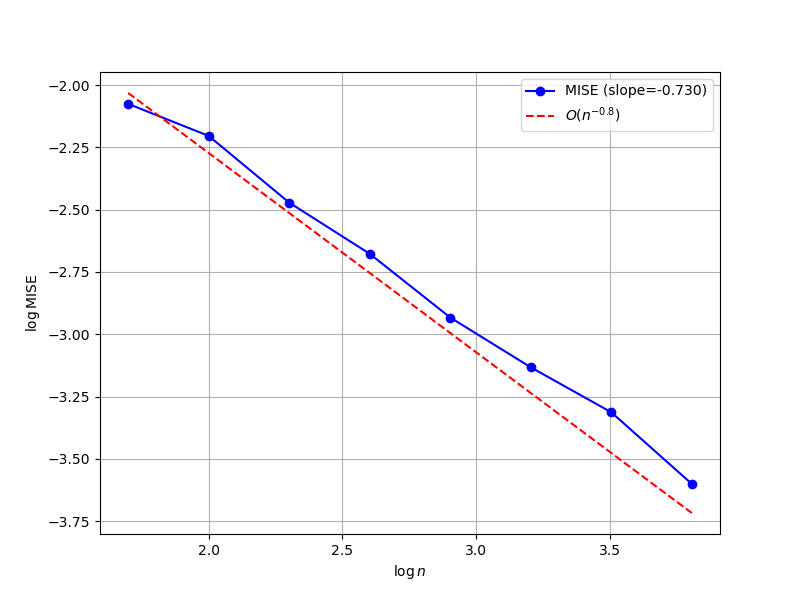
\includegraphics[width=0.6\textwidth]{plot.png}
    \caption{样本量 $n$ 与 MISE 的双对数图}
\end{figure}

实验代码如下：

\begin{lstlisting}[
    language=python,
    basicstyle=\ttfamily,
    breaklines=true，
    commentstyle=\itshape\color{black!50!white}
]

import numpy as np
import matplotlib.pyplot as plt
from scipy.stats import norm, gaussian_kde
from scipy.stats import linregress
np.random.seed(42)

samples = np.array([50, 100, 200, 400, 800, 1600, 3200, 6400]) # 样本量
trials = 100 # 模拟次数

grid = np.linspace(-5, 5, 1000)
dx = grid[1] - grid[0]
density = norm.pdf(grid) # 真实密度函数 N(0,1)

mises = []
for n in samples:
    ises = []
    for _ in range(trials):
        data = np.random.normal(0, 1, n)
        kde = gaussian_kde(data)
        estimated = kde.evaluate(grid) # 核密度估计
        ise = np.sum((estimated - density)**2) * dx 
        ises.append(ise)
    mise = np.mean(ises) # 估算均方误差
    mises.append(mise)

log_n = np.log10(samples)
log_mise = np.log10(mises)
slope, intercept, r_value, p_value, std_err = linregress(log_n, log_mise)
print(f"斜率: {slope:.3f}")
fig = plt.figure(figsize=(8, 6))
plt.plot(log_n, log_mise, 'bo-', label=f'MISE (slope={slope:.3f})')
log_08 = -0.8 * log_n + intercept + (slope - (-0.8)) * log_n[0]
plt.plot(log_n, log_08, 'r--', label='$O(n^{-0.8})$')
plt.xlabel('$\log n$')
plt.ylabel('$\log \mathrm{MISE}$')
plt.legend()
plt.grid(True)
fig.savefig('plot.png')
plt.show()
\end{lstlisting}






\end{document}